% =============================================================================
%  Section: Reconstructed-Track Backgrounds
%  H1 Charged-Hadron SIDIS High-Q^2 Analysis Note
% =============================================================================
\section{Backgrounds}
\label{sec:backgrounds}

The only event-level background arises from DIS events outside the measurement phase space which migrate in due to resolution effects or QED radiation. The phase space of $60 < Q^2< 150$ GeV$^2$ is handled by the high $Q^2$ DJANGOH and RAPGAP MC samples. The region $Q^2 < 60$ GeV$^2$ is handled by a dedicated Djangoh sample, which has negligible contribution in almost all bins. The distributions of this low $Q^2$ background are shown in Fig.~\ref{fig:bg:alpha0p2-reco-background-fractions}. The background from $Q^2 < 4$ GeV$^2$ (including photoproduction) was evaluated with Pythia and found to be negligible, only 5 photoproduction events are expected in the whole event sample. Similarly, the contribution from exclusive vector meson production was studied with DIFFVM elastic $\rho$ production.  Its integrated contribution is negligible, $0.0074\%$ of the reconstructed-track denominator, but it is bin-localized at high $z$: the $z$ row $0.7\le z<1.0$ reaches $2.18\%$ and the worst single cell $4.53\%$.  The measured elastic-$\rho$ contribution is reserved as a systematic-only, source-distinct template; it is not subtracted per bin and is not part of the current systematic budget.  The $\phi$ and $\omega$ channels and proton-dissociative $\rho$ production remain unquantified caveats.  For this analysis, diffractive DIS is not subtracted.

After the charged-SIDIS event and track
selection, two non-negligible reconstructed-track background categories are
considered in the current high-$\Qsq$ analysis:
\begin{enumerate}
  \item electron and positron tracks, including tracks from Dalitz decays or
        semi-leptonic decays of mesons;
  \item charged tracks arising from decays of long-lived neutral hadrons.
\end{enumerate}


The electron background category is modeled by selecting reconstructed electrons or positrons in DJANGOH and RAPGAP. This background arises from photon conversions, hadron decays, or tracks from scattered electrons or positrons which are not properly matched to their calorimeter cluster. The mis-identified scattered-electron background is reduced by rejecting tracks within $0.2$ radians of the nominal scattered-electron three-vector, which can come from the calorimeter cluster; accepted tracks satisfy
$\alpha(\mathrm{track},e')\ge0.2~\mathrm{rad}$. The remaining $e^\pm$ background arises mainly from meson decays and lives mostly at low-$z$.
Since the cone-baseline promotion of 2026-10-13 this requirement is part of
the central selection rather than a diagnostic variant; cone-rejected matched
legs flow to the miss row of the response.

The V0 decay daughter category is identified through the absolute value of
a multi-hop search for a V0 PDG code.  The exact ancestor set used is
\begin{equation}
  |\mathrm{PDG}_{\mathrm{ancestor}}| \in \{310,\;130,\;311,\;3122\}\, ,
\end{equation}
corresponding to $K^{0}_{S}$, $K^{0}_{L}$, $K^{0}/\bar K^{0}$, and
$\Lambda/\bar\Lambda$ ancestors.  This is the definition used to remove background from V0s.

In the current response, the detector-interaction removable
class is removed response-internally through an enlarged per-reco-bin fake
fraction $f_i$ (pooled removable fraction $0.9096$), while charged kaons
from detector interactions with a reconstructed parent are kept as signal.  An
external subtraction of the detector-interaction component is therefore
forbidden: it would double-remove the class.  Electrons and V0 daughters are
in addition vetoed at the selection level, and their residual contamination,
together with the low-$\Qsq$ leakage, is subtracted from the data vector
before unfolding using the Monte Carlo background templates; the total
subtracted content is $281{,}250.09$ tracks, $7.2767\%$ of the cone data
vector.

The current canonical reco-background fraction display is shown in
Fig.~\ref{fig:bg:alpha0p2-reco-background-fractions}.  The fraction is defined
as the expected background-track count divided by the reconstructed-track
count after the $\alpha<0.2$ selection in the same
$(\Qsq,x,z,\pTh,\mathrm{charge})$ bin. The plotted
components are the residual $e^\pm$ background, the matched-V0-daughter
background, the low-$\Qsq$ component, and their total where shown. The integrated reco track count is $3{,}865{,}073$, of which the estimated track-level background total at $\mathcal{L}=351000.0~\nbinv$ is $308{,}655.9$ ($7.986\%$), split into $148{,}976.4$ electron and positron tracks, $132{,}065.3$ V0 decay daughters, $27{,}405.8$ detector-interaction secondaries, and $208.4$ low-$\Qsq$ leakage tracks, with the $e^\pm$ and V0 components located mostly at low $z$.
Of these four categories, the electron, V0, and low-$\Qsq$ components are the
ones subtracted from the data vector before unfolding in the current release;
the detector-interaction component is not subtracted externally but removed
response-internally, as described above.

The curves for the $e^\pm$ and V0 backgrounds are taken as the average of DJANGOH and RAPGAP.

\begin{figure}[p]
  \centering
  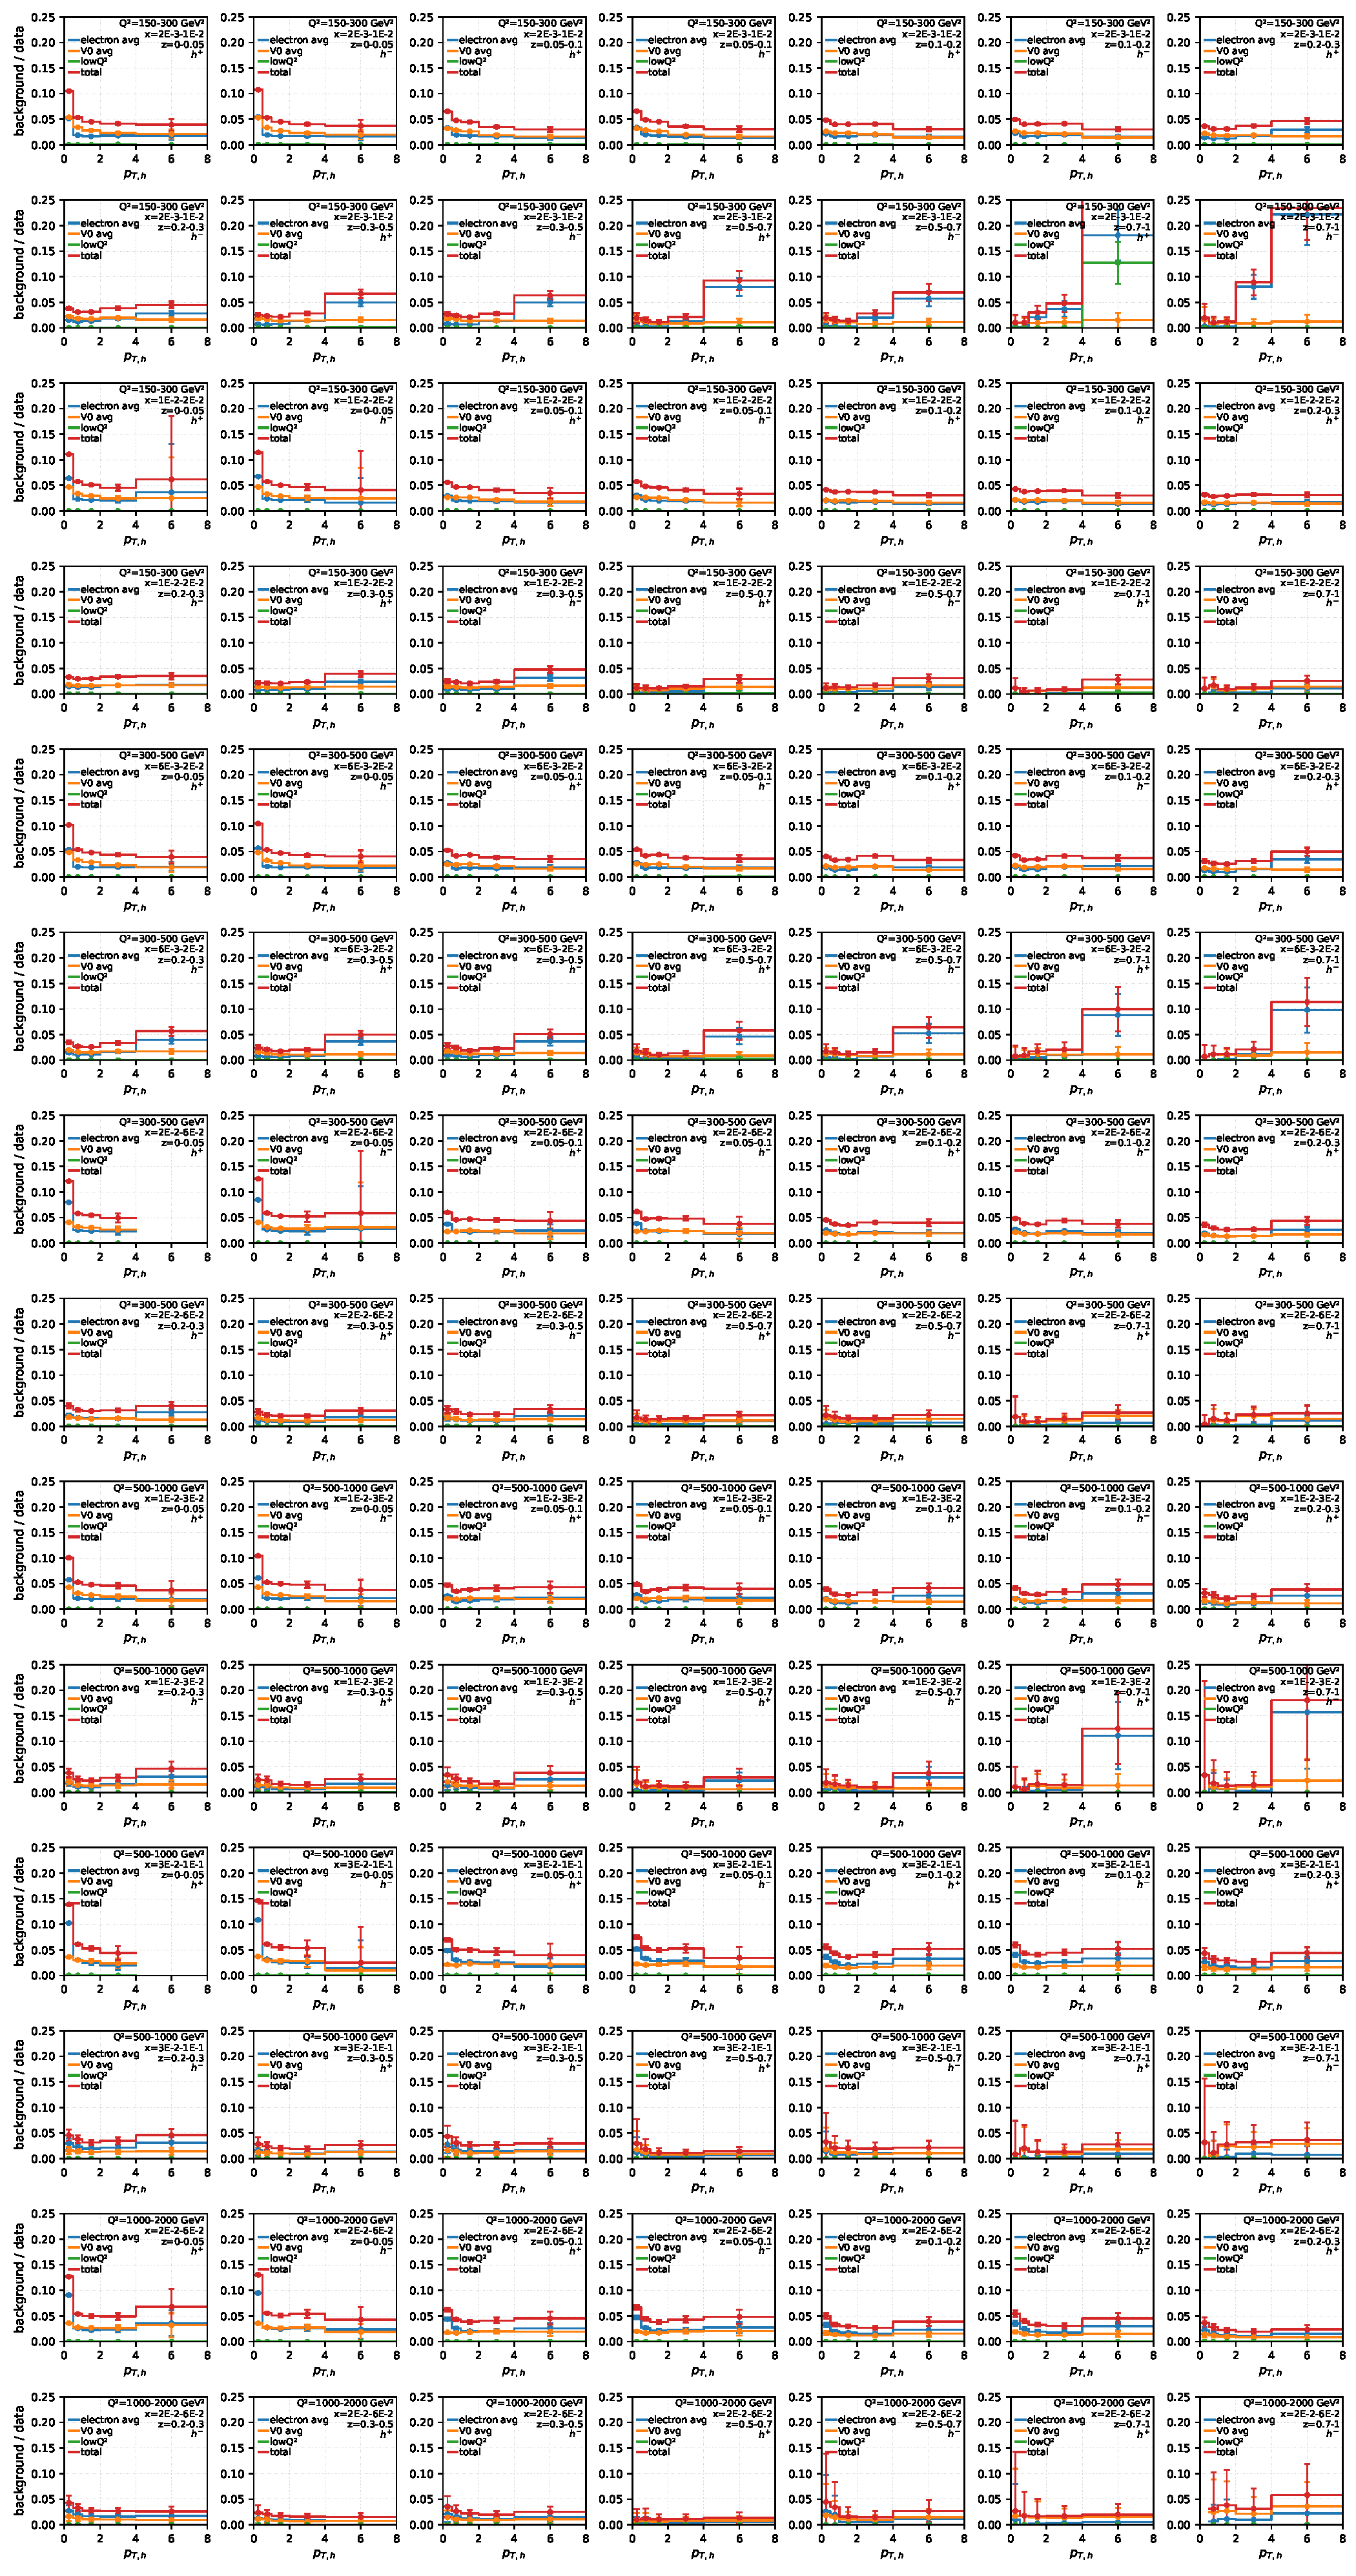
\includegraphics[width=0.95\textwidth,height=0.9\textheight,keepaspectratio]{figures/fig_reco_background_fractions_alpha0p2_onepage_7col.pdf}
  \caption{Reco-level background fractions after the $\alpha<0.2$ selection,
  defined as the number of background tracks divided by the number of reco tracks in the same
  $(\Qsq,x,z,\pTh,\mathrm{charge})$ bins.  The
  first column corresponds to $0.0 \le z < 0.05$.}
  \label{fig:bg:alpha0p2-reco-background-fractions}
\end{figure}

As a complementary diagnostic display of the background model,
Figs.~\ref{fig:bg:reco-multiplicity-dist-per-cell}
and~\ref{fig:bg:reco-multiplicity-dist-combined} show the raw, uncorrected
per-event multiplicity distributions of reconstructed charged hadrons in the
seven $(\Qsq,x)$ cells of Table~\ref{tab:binning:z005-contract}, with the
per-source background expectations overlaid.  The event sample is the
analysis-fiducial selection of Sec.~\ref{sec:selection:final-events}:
$0.1<y_{e\Sigma}<0.7$, $E-p_z>45~\GeV$, $150<\Qsq<20000~\GeVsq$, and
$|z_{\mathrm{vtx}}|<35~\mathrm{cm}$.  The overlaid expectations are expected
event counts at $\mathcal{L}=351000.0~\nbinv$ ($351~\pbinv$) from the
alpha0p2 background chain, shown separately for four sources: electron
tracks, V0 decay daughters, detector-interaction secondaries, and
low-$\Qsq$ leakage (fid-gate overlay variant).  Each background curve is
displayed as expected events versus the number of that source's background
tracks per event; its $n=0$ entry is the fiducial event population
containing none of that source.  The background model is
diagnostic/provisional and is not a physics-approved subtraction.  The
figures, their input tables, and the $n=0$ convention are documented in the
figure package \path{sidis_highQ2/plots/reco_multiplicity_note_2026-10-07/}
(README.txt); the data input tables are the v6 fid-variant study outputs
\path{H1ChargedSidis_HighQ2/output_v6/studies/reco_multiplicity_dist_2026-10-07/}
and
\path{H1ChargedSidis_HighQ2/output_v6/studies/reco_multiplicity_dist_combined_2026-10-08/},
and the background input table is
\path{H1ChargedSidis_HighQ2/output_v6/studies/reco_backgrounds_multdist_2026-10-07/aggregate/background_multdist_per_cell_L351000.csv}.

\begin{figure}[p]
  \centering
  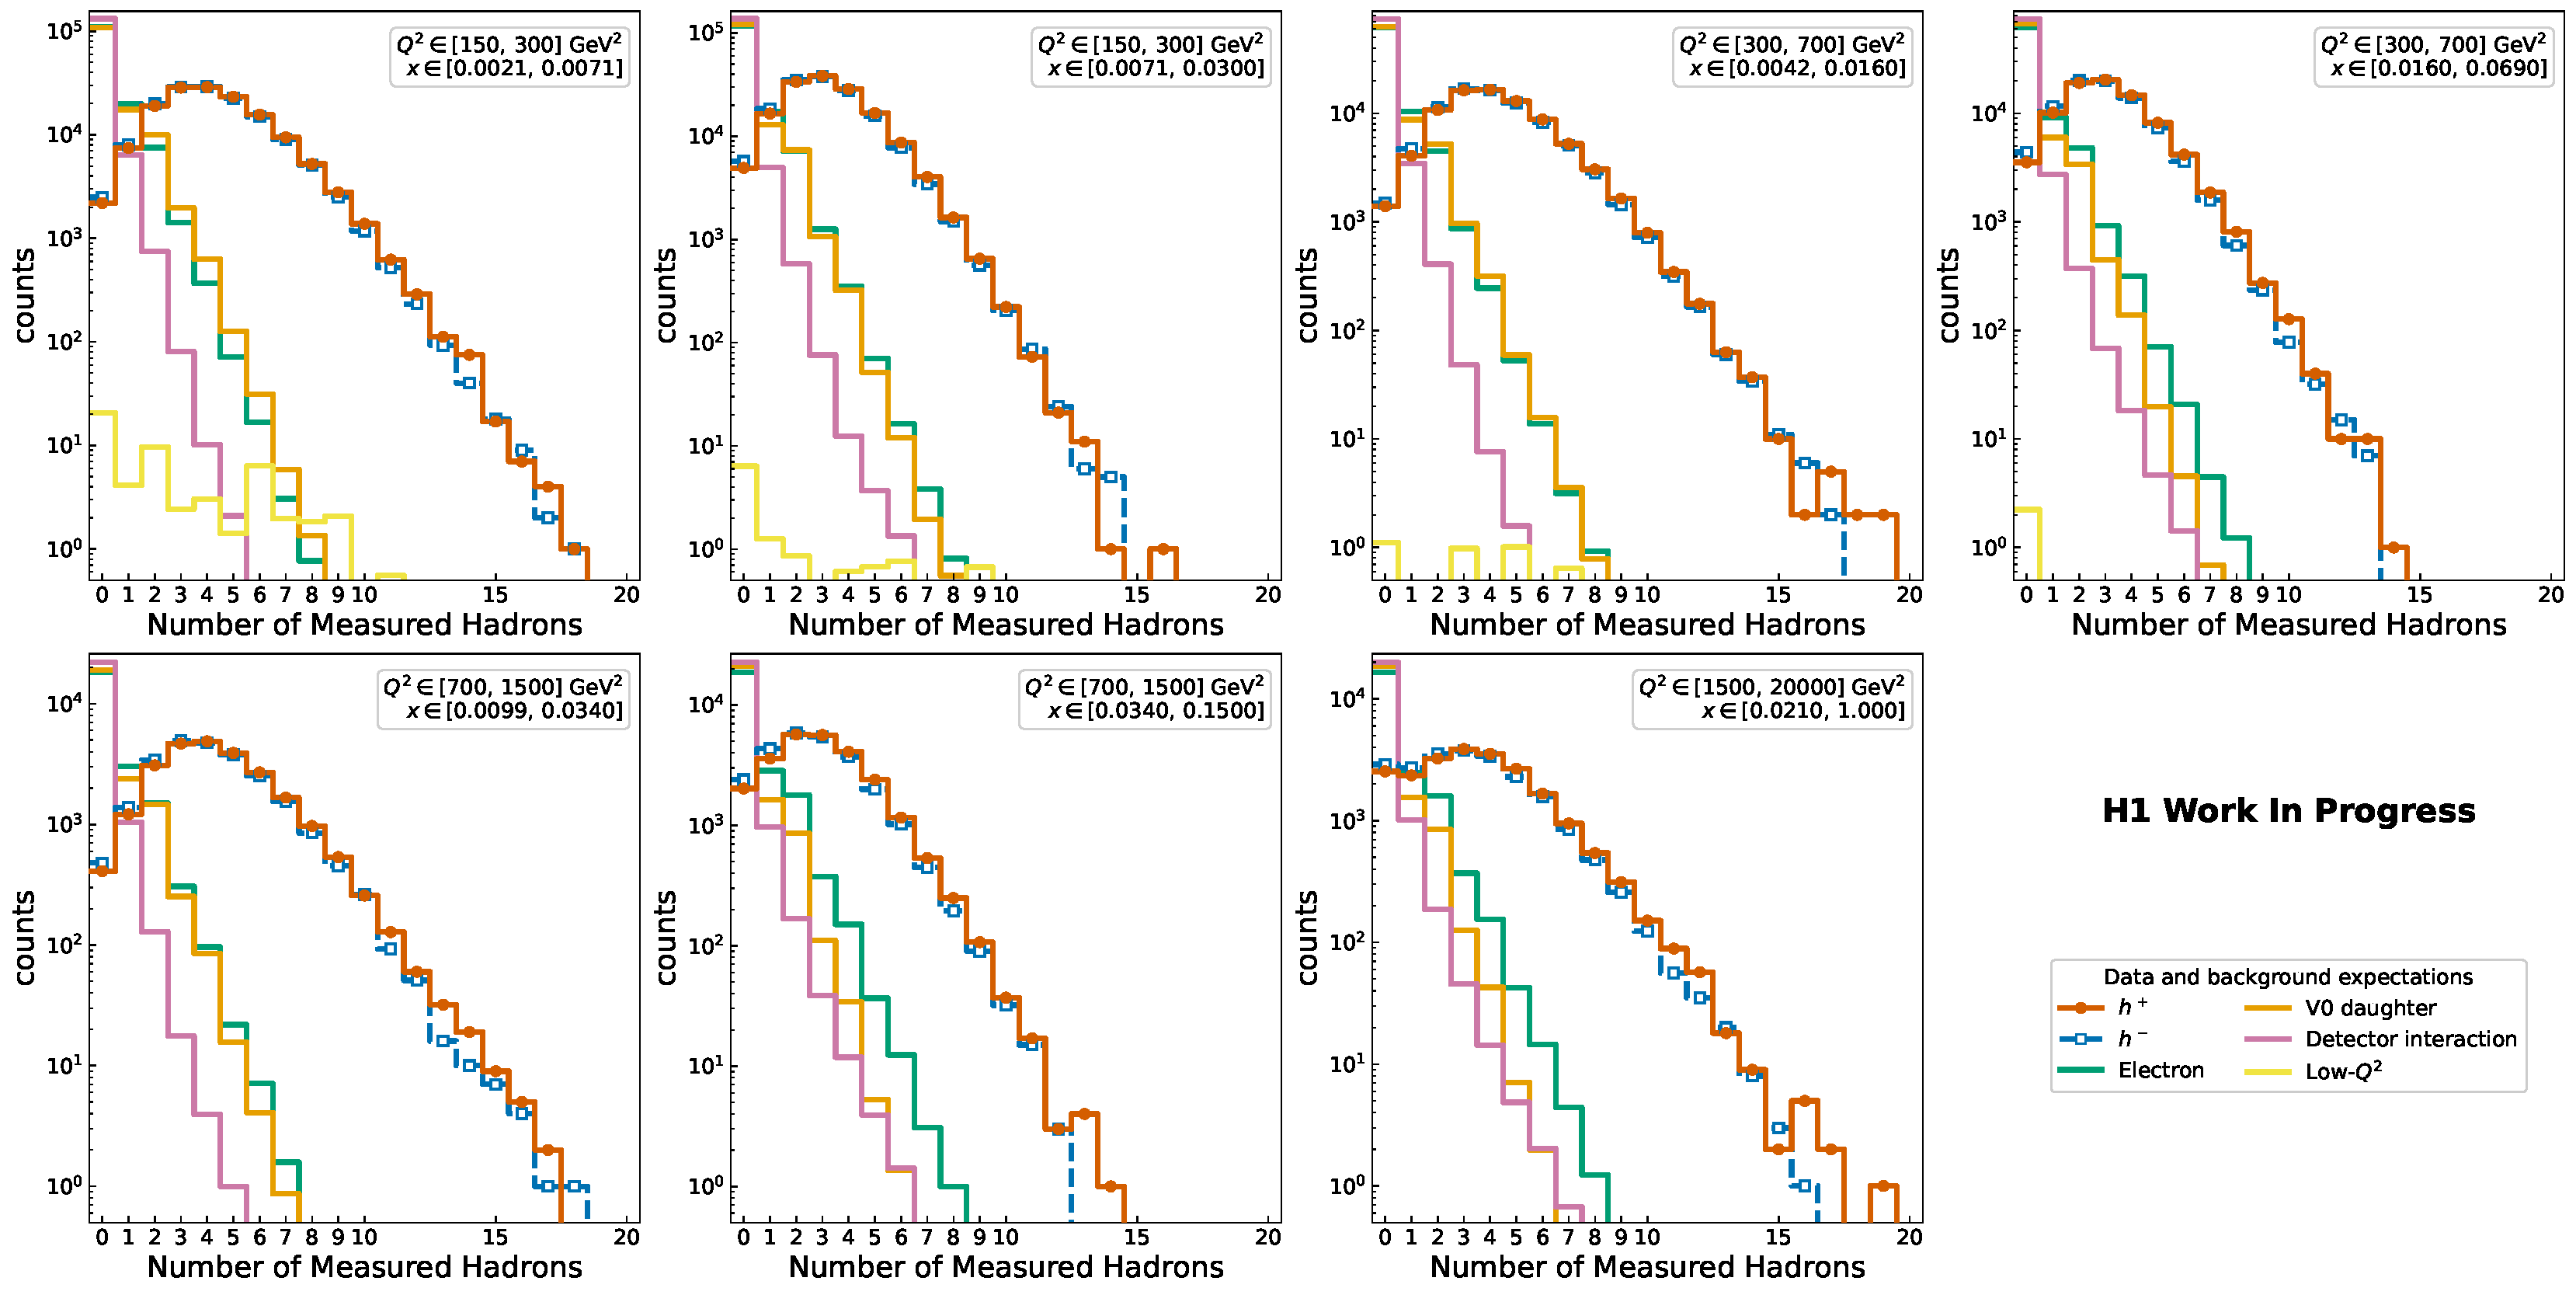
\includegraphics[width=0.98\textwidth,height=0.82\textheight,keepaspectratio]{figures/fig_reco_multiplicity_dist_per_cell_hQ2_v6data_20261007.pdf}
  \caption{Raw, uncorrected per-event multiplicity distributions of
  reconstructed charged hadrons in the seven $(\Qsq,x)$ cells for the
  analysis-fiducial event selection ($0.1<y_{e\Sigma}<0.7$,
  $E-p_z>45~\GeV$, $150<\Qsq<20000~\GeVsq$,
  $|z_{\mathrm{vtx}}|<35~\mathrm{cm}$), shown on a logarithmic y-axis.
  $\hplus$ (filled circles) and $\hminus$ (open squares) are shown
  separately in each cell.  Overlaid are the background expectations at
  $\mathcal{L}=351000.0~\nbinv$ ($351~\pbinv$) from the alpha0p2 background
  chain -- electron, V0 daughter, detector-interaction secondaries, and
  low-$\Qsq$ leakage (fid-gate overlay variant) -- each as expected events
  versus the number of that source's background tracks per event; the $n=0$
  entry of each background curve is the fiducial event population containing
  none of that source.  The background model is diagnostic/provisional.}
  \label{fig:bg:reco-multiplicity-dist-per-cell}
\end{figure}

\begin{figure}[p]
  \centering
  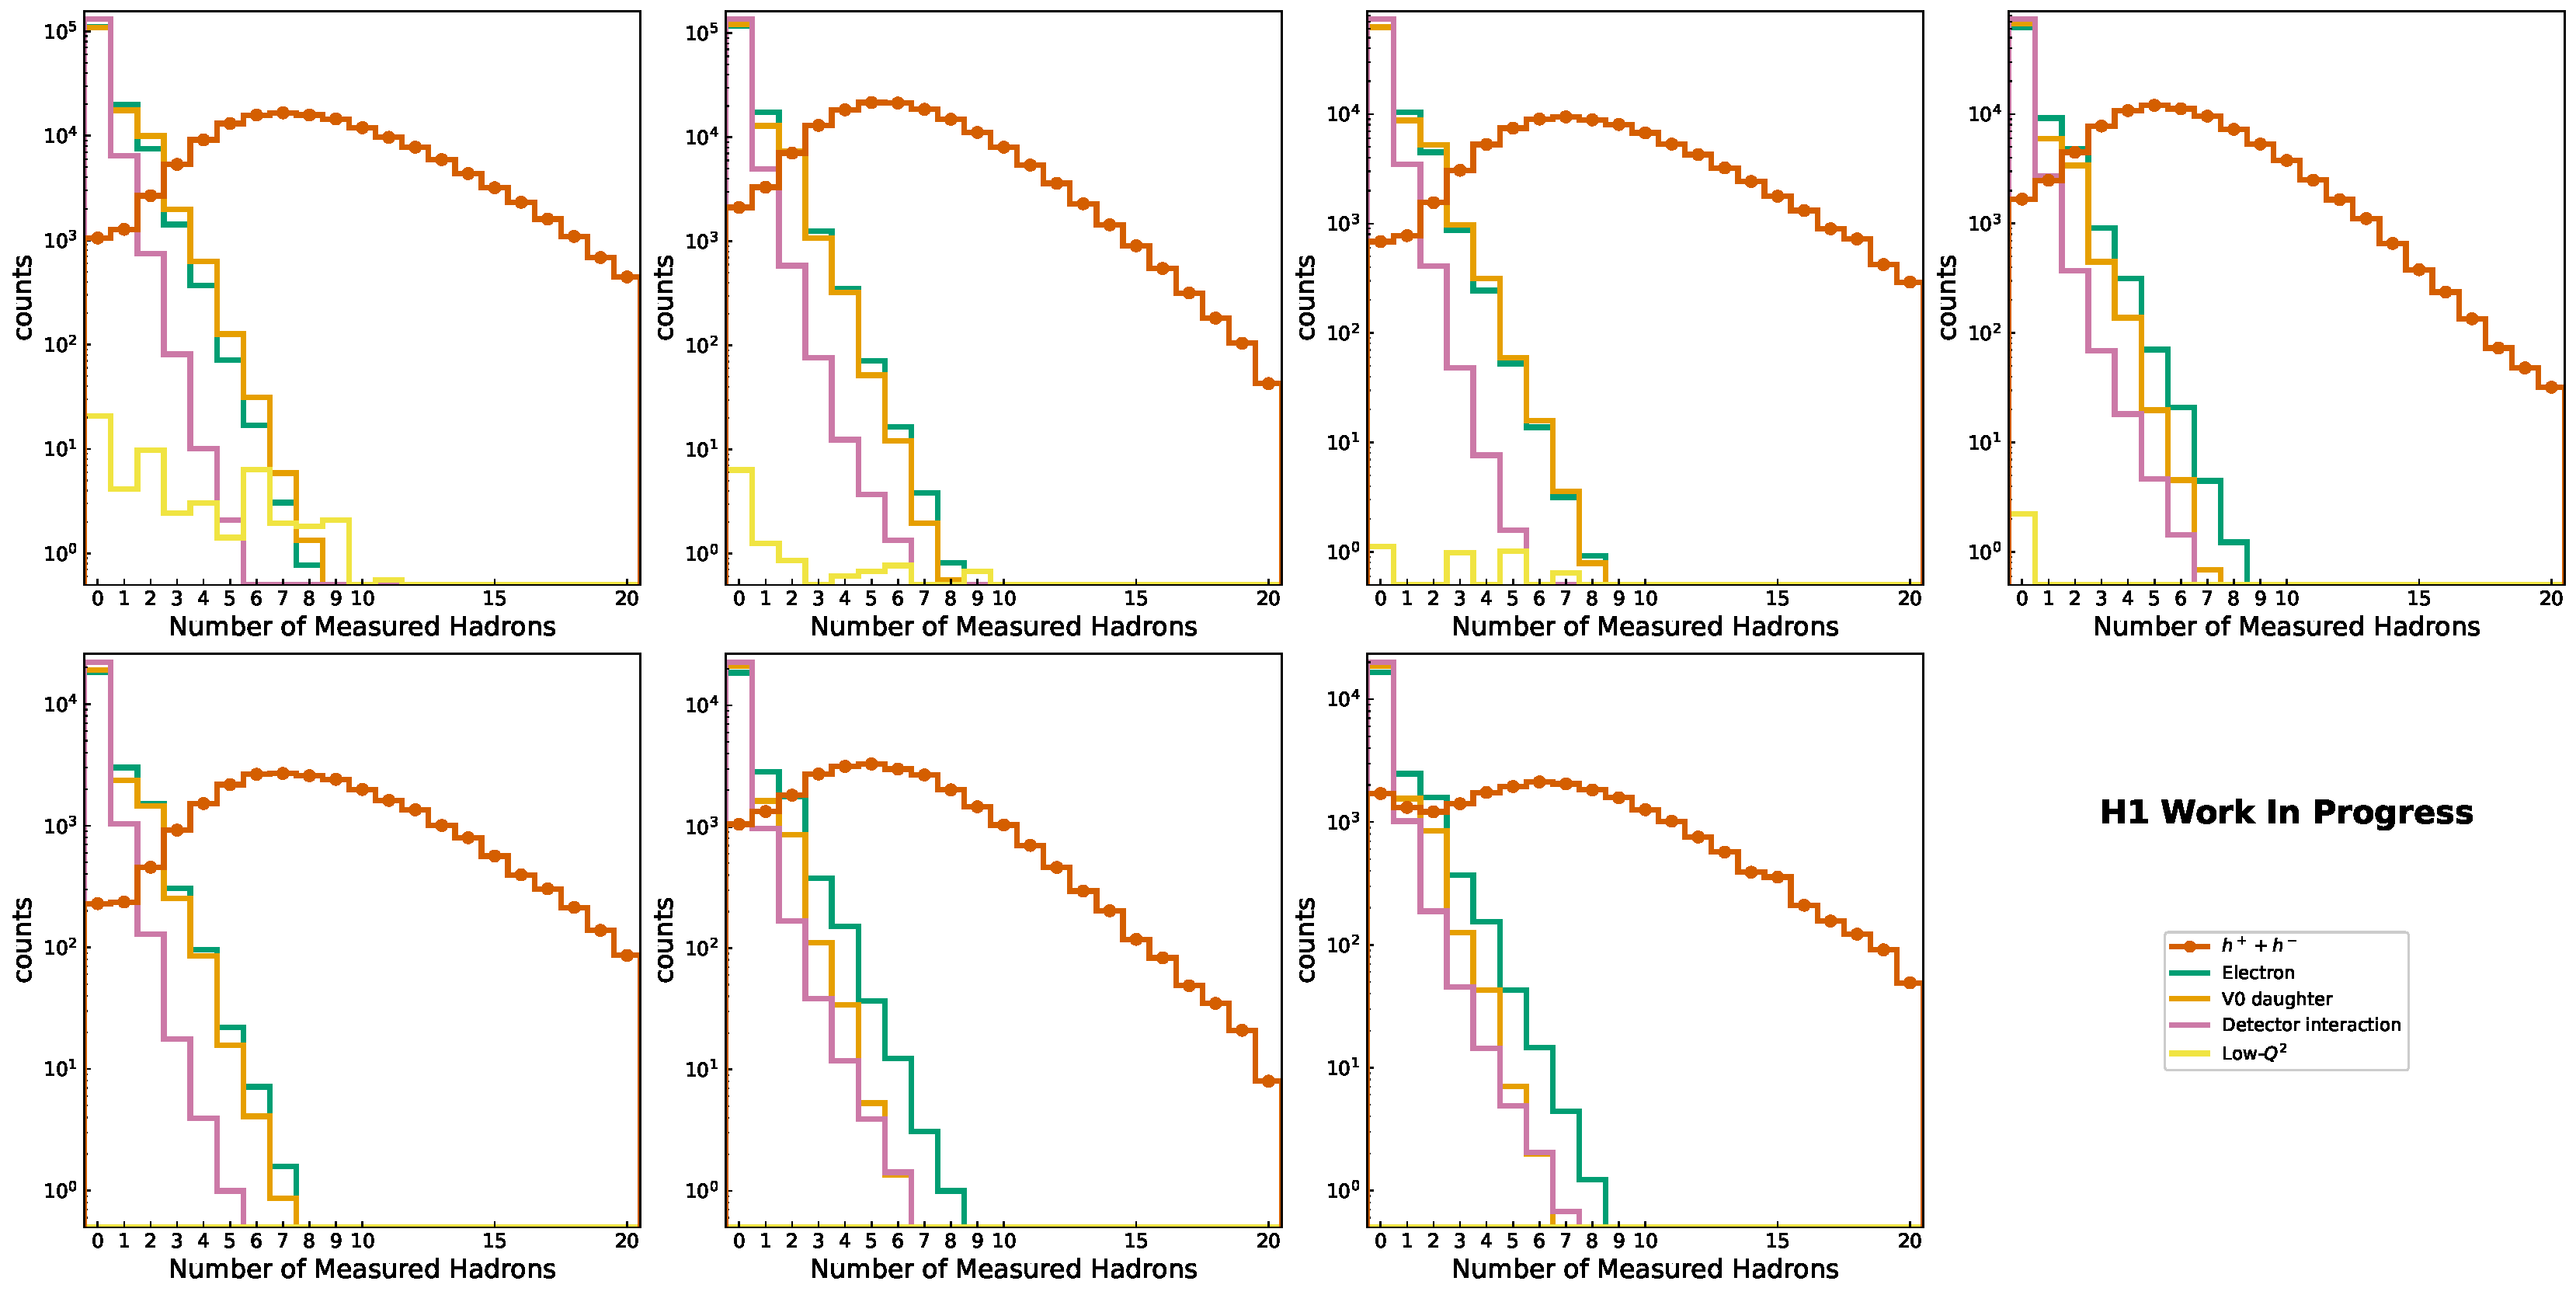
\includegraphics[width=0.98\textwidth,height=0.82\textheight,keepaspectratio]{figures/fig_reco_multiplicity_dist_per_cell_combined_hQ2_v6data_20261008.pdf}
  \caption{Raw, uncorrected per-event total charged-hadron multiplicity
  $n_{\hplus}+n_{\hminus}$ in the seven $(\Qsq,x)$ cells for the
  analysis-fiducial event selection ($0.1<y_{e\Sigma}<0.7$,
  $E-p_z>45~\GeV$, $150<\Qsq<20000~\GeVsq$,
  $|z_{\mathrm{vtx}}|<35~\mathrm{cm}$), shown on a logarithmic counts axis;
  each event is counted once at its total $n_{\hplus}+n_{\hminus}$.  Events
  with $n\ge21$ are excluded from the $0$--$20$ axis; the excluded event
  counts are S0\_x0: 818, S1\_x0: 520, S2\_x0: 213, S3\_x0: 144,
  S0\_x1: 60, S1\_x1: 35, and S2\_x1: 14.  Overlaid are the
  background expectations at $\mathcal{L}=351000.0~\nbinv$
  ($351~\pbinv$) from the alpha0p2 background chain -- electron, V0
  daughter, detector-interaction secondaries, and low-$\Qsq$ leakage
  (fid-gate overlay variant) -- each as expected events versus the number of
  that source's background tracks per event; the $n=0$ entry of each
  background curve is the fiducial event population containing none of that
  source.  The background model is diagnostic/provisional.}
  \label{fig:bg:reco-multiplicity-dist-combined}
\end{figure}
